\begin{problem}{Zhuangba and Triangle}{standard input}{standard output}{1 second}{512 megabytes}

% 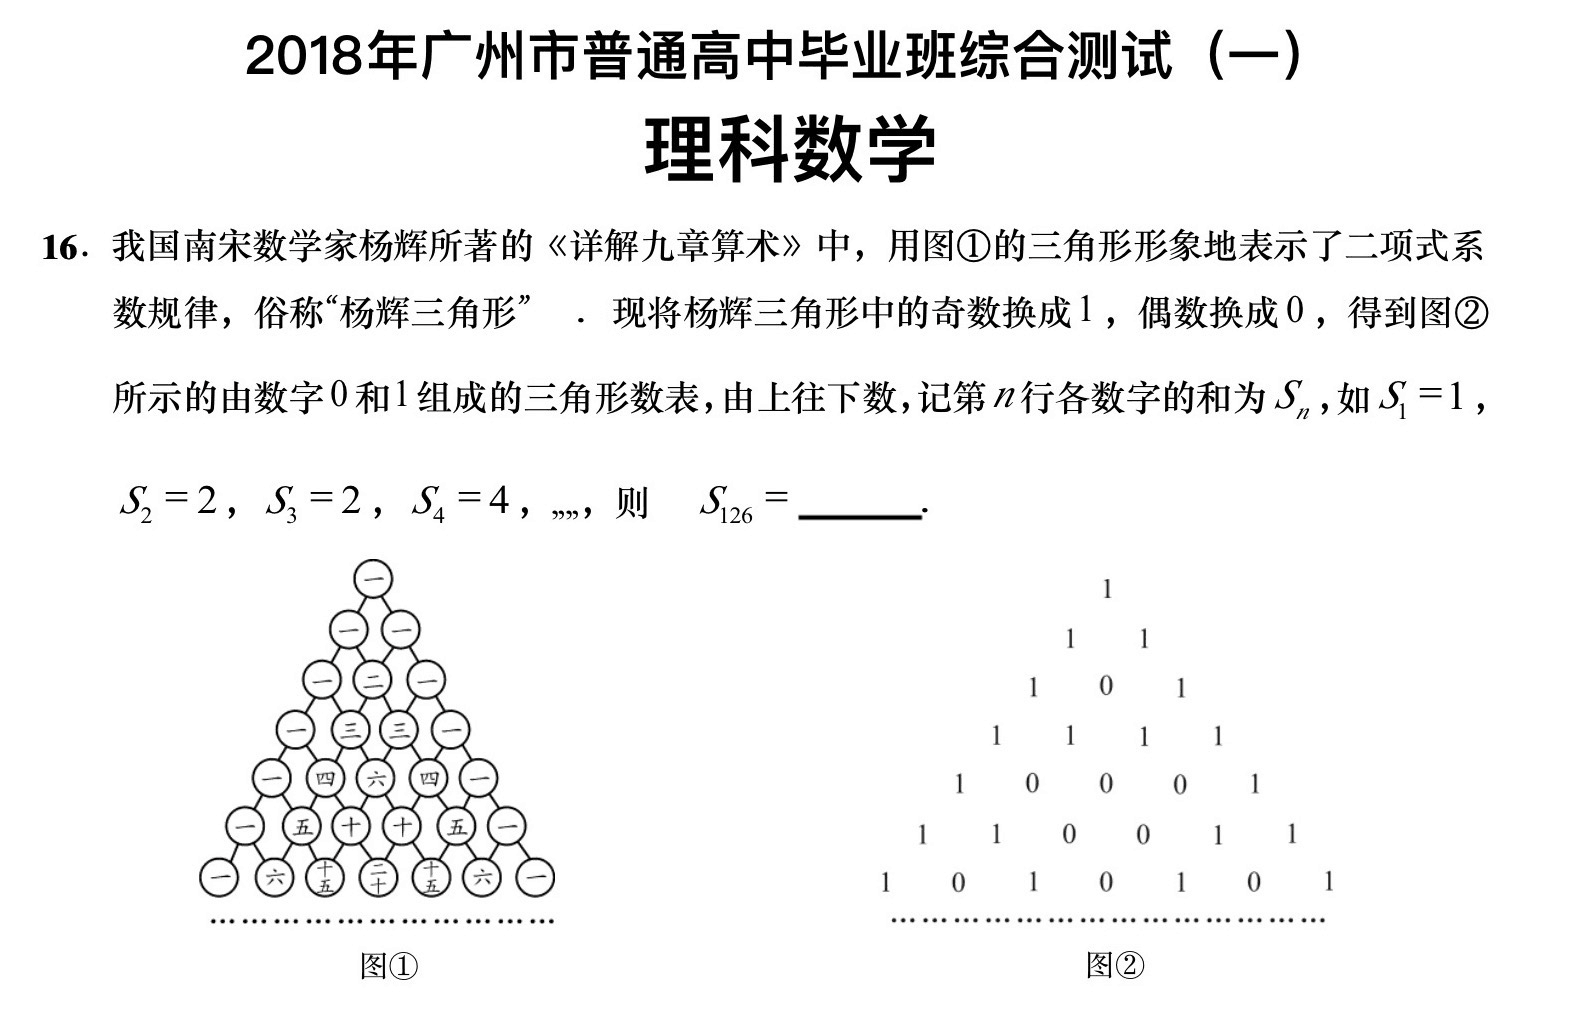
\includegraphics[width=0.25\textwidth]{aa.png}%

强如 $Zhuangba$ 也需要做一些模拟题。

在 2020年5月20日 下午五点 她在全班数学模拟考时候做到这样一道模拟题。

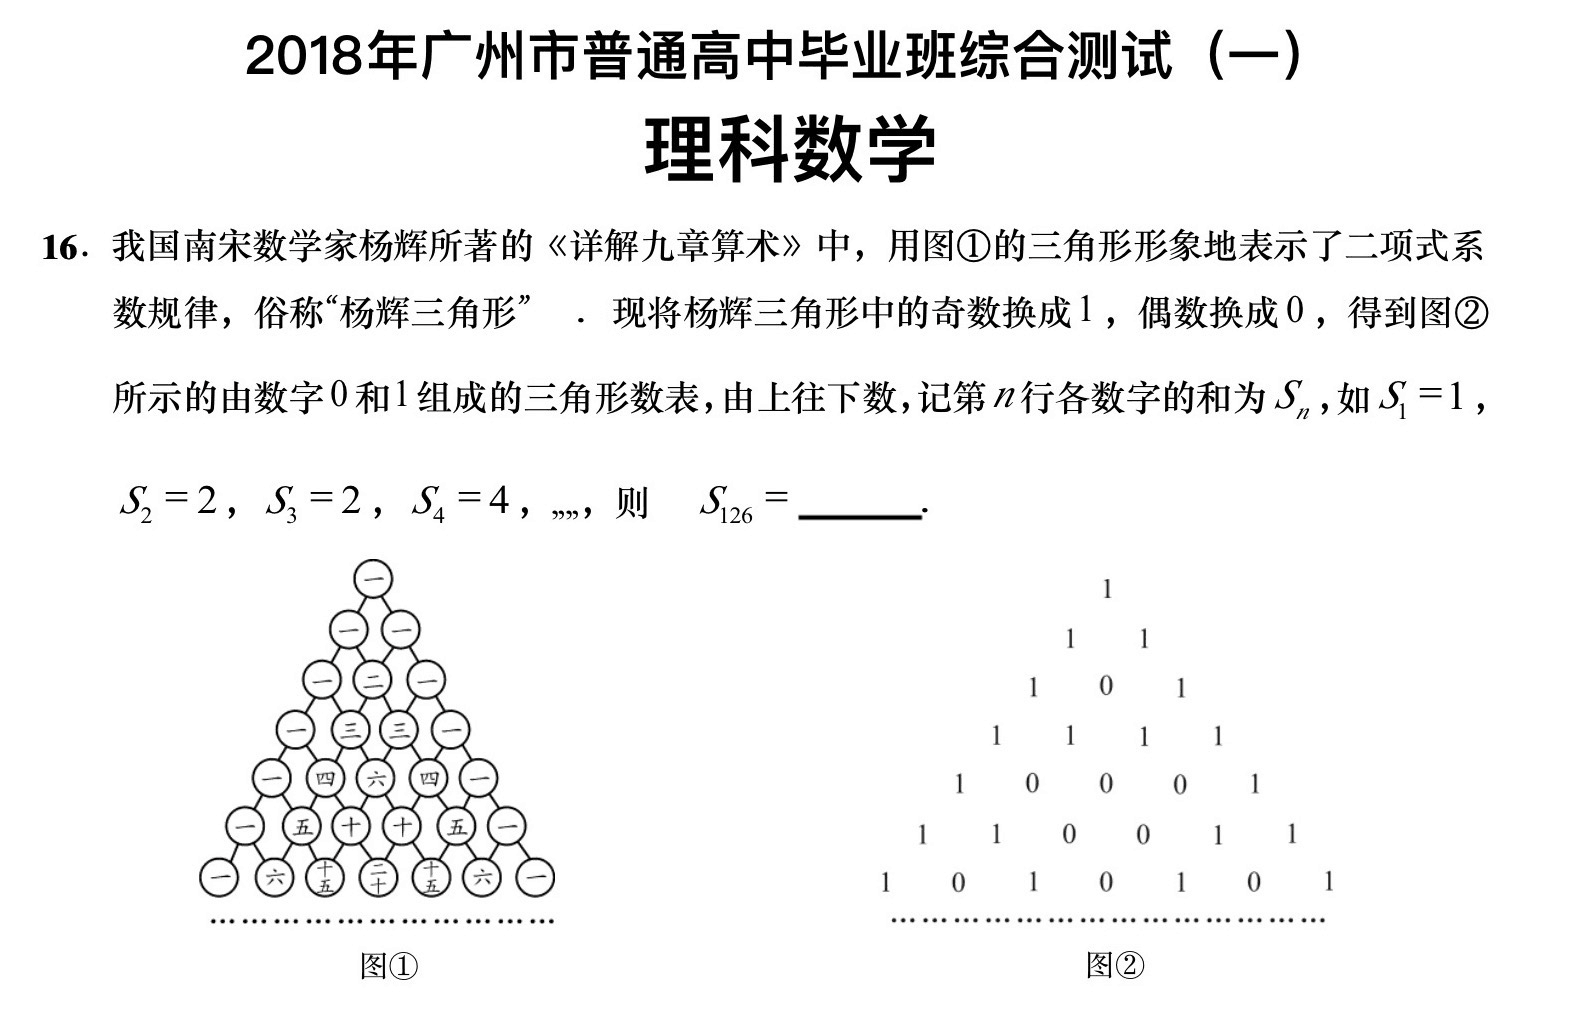
\includegraphics[width=0.95\textwidth]{aa.png}%


但这显然太简单了不是嘛? 善于思考的 Zhuangba 想到了另一个有趣的问题:能不能快速知道杨辉三角第$n$行的每个数 \% 2 之后的结果。

\InputFile

输入一个数字 $n(1\le n \le 10^6)$, 表示需要求的杨辉三角的第$n$行 \% 2 的结果。

\OutputFile

输出Pascal Triangle第$n$行的 \% 2 的结果,每个数之间用空格间隔开。

\Example

\begin{example}
\exmpfile{example.1.in}{example.1.ans}%
\exmpfile{example.2.in}{example.2.ans}%
\end{example}

\end{problem}
